
\subsubsection{Reactants}

\subsubsubsection{\texttt{FreeChemical}}

\texttt{FreeChemical} simply represents a pool of interchangeable molecules distributed uniformly in the cell. Computationnally, only the number of molecules in the pool is relevant.

\subsubsubsection{\texttt{BoundChemical}}

\begin{figure}[!h]
  \centering
  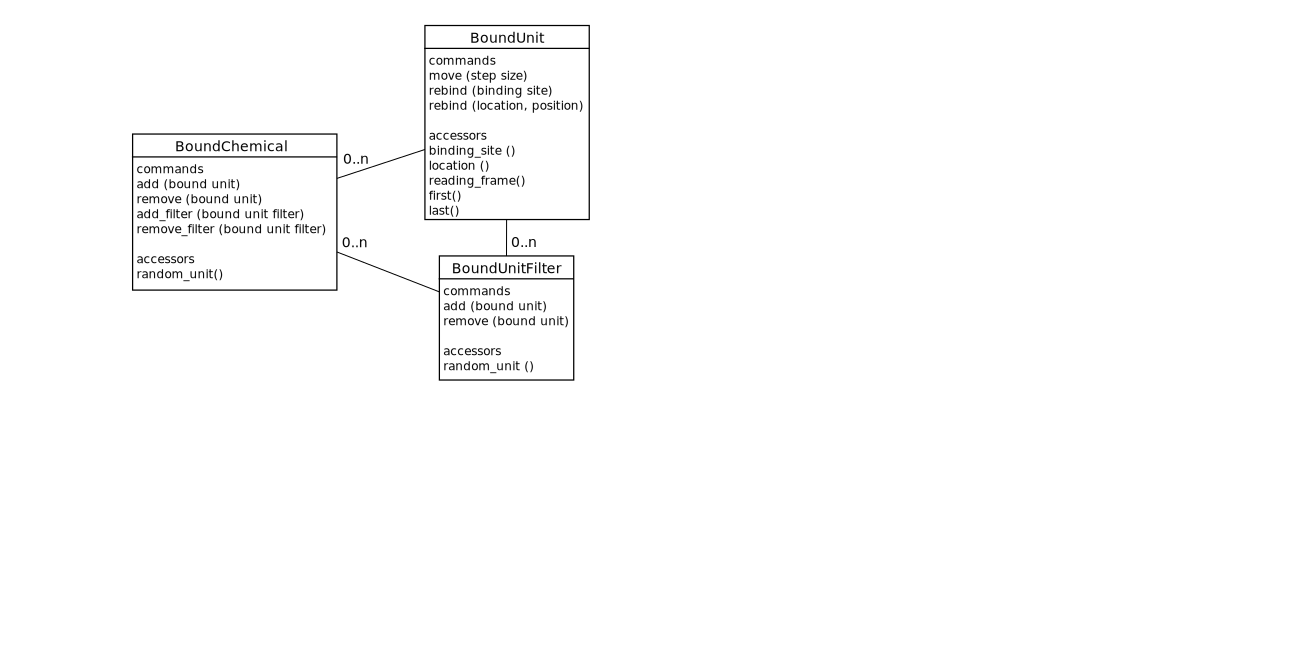
\includegraphics[width=\linewidth]{boundchemical}
  \caption{\texttt{BoundChemical} are in fact a pool of individual \texttt{BoundUnit} created using a \texttt{BoundUnitFactory}. A \texttt{BoundUnit} is characterized by the \texttt{ChemicalSequence} it bound to and its current position. Reaction then use \texttt{BoundUnitFilter} to sort \texttt{BoundUnit} according to some criterium of reference (\textit{e.g.} \texttt{Loading} reactions sort \texttt{BoundUnit} according to the motif they read).}
  \label{fig:det_bound_chemical}
\end{figure}

\texttt{BoundChemical} represents molecules of the same chemical species, but there are specifities for each unit of a \texttt{BoundChemical}, as all units are bound at different locations of different \texttt{ChemicalSequence}~\reffigp{fig:det_bound_chemical}. A \texttt{BoundUnitFactory} is used to recycle \texttt{BoundUnit}s, avoiding memory reallocation throughout simulation. \texttt{BoundUnitFilters} are used to sort \texttt{BoundUnit}s according to criteria useful for reactions~\reffigp{fig:det_bound_chemical}.


\texttt{BoundUnit}s are passed from one \texttt{BoundChemical} species to another through reactions, their attributes are updated if needed. They are only destroyed once they are unbound from their \texttt{ChemicalSequence}.

\subsubsubsection{\texttt{ChemicalSequence}}

\begin{figure}[!h]
  \centering
  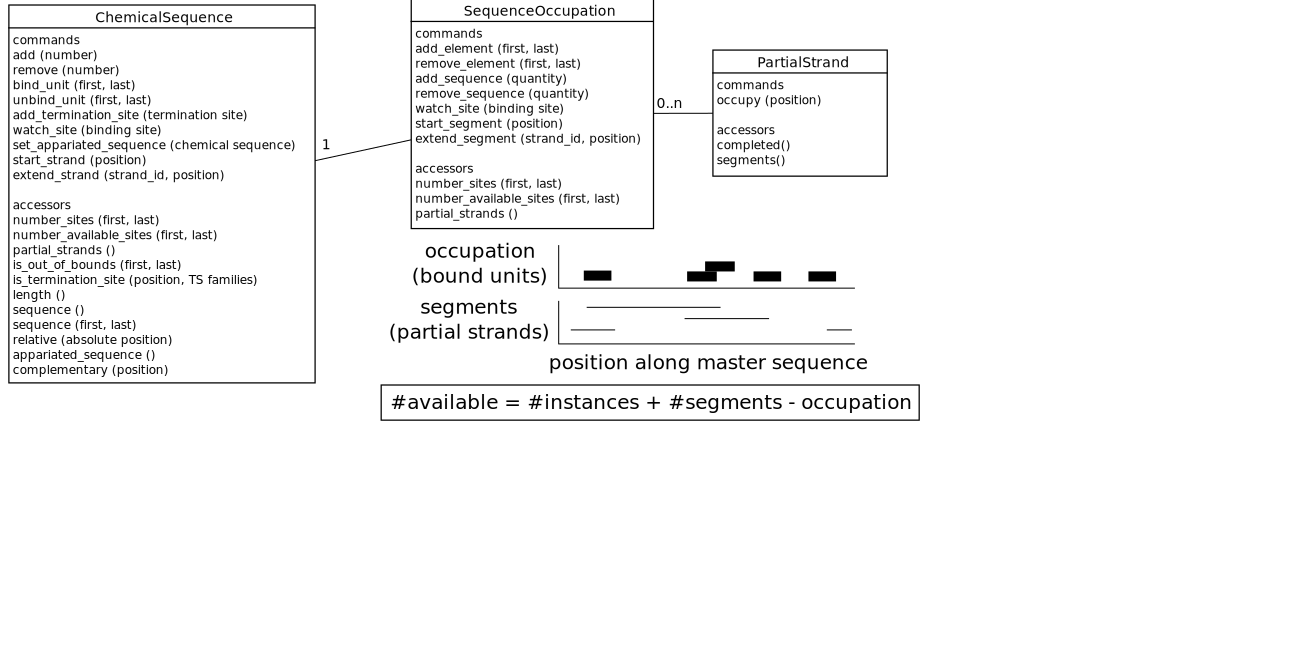
\includegraphics[width=\linewidth]{chemicalsequence}
  \caption{\texttt{ChemicalSequence} represents a pool of polymeres that can be elongated and on which \texttt{BoundUnit}s bind through \texttt{BindingSite}s. For binding to occur, availability of \texttt{BindingSite} is assessed using a utility class \texttt{SequenceOccupation} that records the number of instances of the polymer, the position of \texttt{BoundUnit}s and elongation of \texttt{PartialStrand}s. \texttt{SiteGroup} is used to notify sites of availability changes more efficiently.}
  \label{fig:det_chemical_sequence}
\end{figure}

\texttt{ChemicalSequence} handles a pool of polymers. A pool is defined by a \emph{master sequence} describing what a typical polymer looks like (\textit{e.g.} the sequence of DnaA protein) and the number of \emph{instances} of the master sequence in the pool. For efficiency reason, we do the following assumptions.

\paragraph{Simplifying assumptions}
\begin{itemize}
\item No deviation from master sequence, all instances are identical.
\item \texttt{BoundUnit}s are not assigned to a specific instance of the sequence, they are positioned on the  master sequence.
\end{itemize}

\subparagraph{Consequences}
\begin{itemize}
\item No direct inference of collisions is possible.
\item A chemical can bind on a partial strand, yet move along the whole sequence freely.
\item Degradation of an instance does not cause unbinding.
\end{itemize}

\paragraph{Site availability}
Despite our simplifying assumptions it is still possible to provide an accurate description of site availability. Availability depends of the number of sequences, number and position of bound elements, number and position of newly polymerized sequence segments~\reffigp{fig:det_chemical_sequence}.

\subsubsubsection{\texttt{DoubleStrand}}

\begin{figure}[!h]
  \centering
  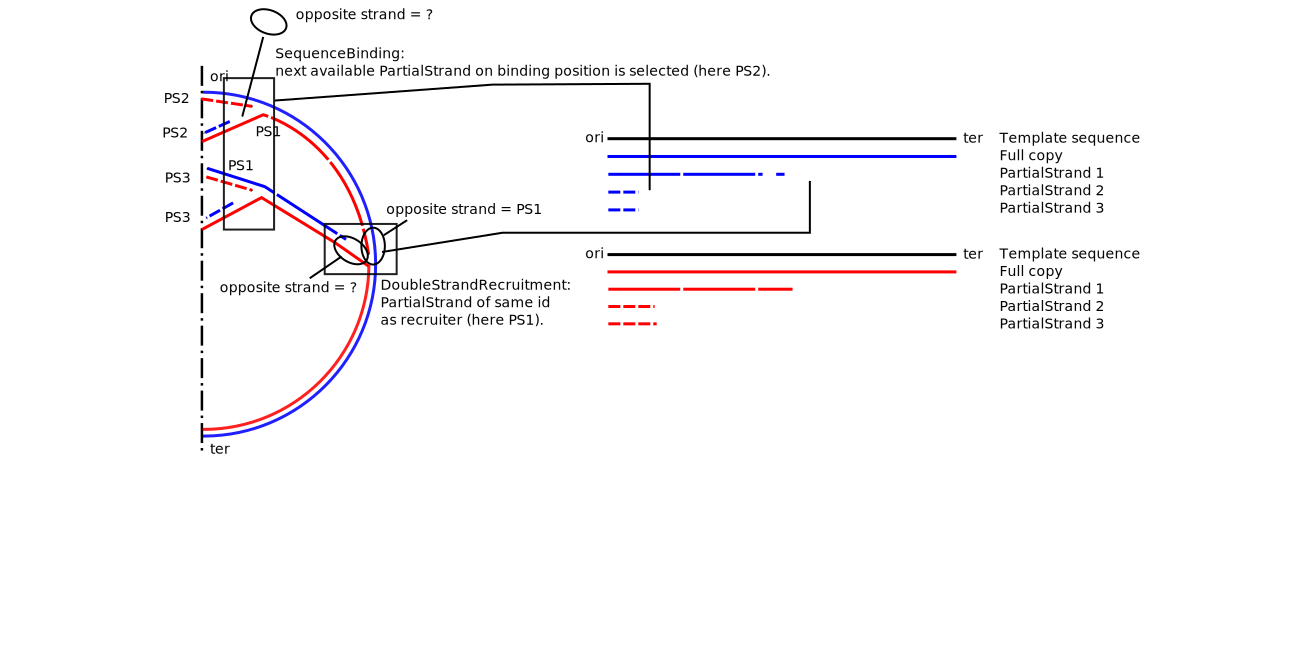
\includegraphics[width=\linewidth]{strand_id}
  \caption{Strands of a \texttt{DoubleStrand} are identified according to creation order. Every time a new segment is polymerized, it is necessary to determine which \texttt{PartialStrand} is elongated. If a polymerase has been recruited on the complementary strand by \texttt{DoubleStrandRecruitment}, it is automatically assigned the same partial strand as the recruiter.}
  \label{fig:strand_id}
\end{figure}

\paragraph{Strand identification} Because \texttt{DoubleStrand} typically reprensents DNA, we expect that the \texttt{DoubleStrand} will contain a lot of \texttt{PartialStrand}s. For replication, it is important to know exactly which strand are opposite to one another for \texttt{DoubleStrandRecruitment} to work properly. We use strand identification as shown in~\reffigt{fig:strand_id}.


\subsubsubsection{\texttt{BindingSiteFamily}}

The task of a \texttt{BindingSiteFamily} is to regroup all the binding sites that can participate in a same \texttt{SequenceBinding} reaction. To simplify the reaction, it stores the subrate associated with each binding site. In order to update the rate properly when availability of sites changes, an \emph{observer pattern} is used~\reffigp{fig:det_bsf}. 

\begin{figure}[!h]
  \centering
  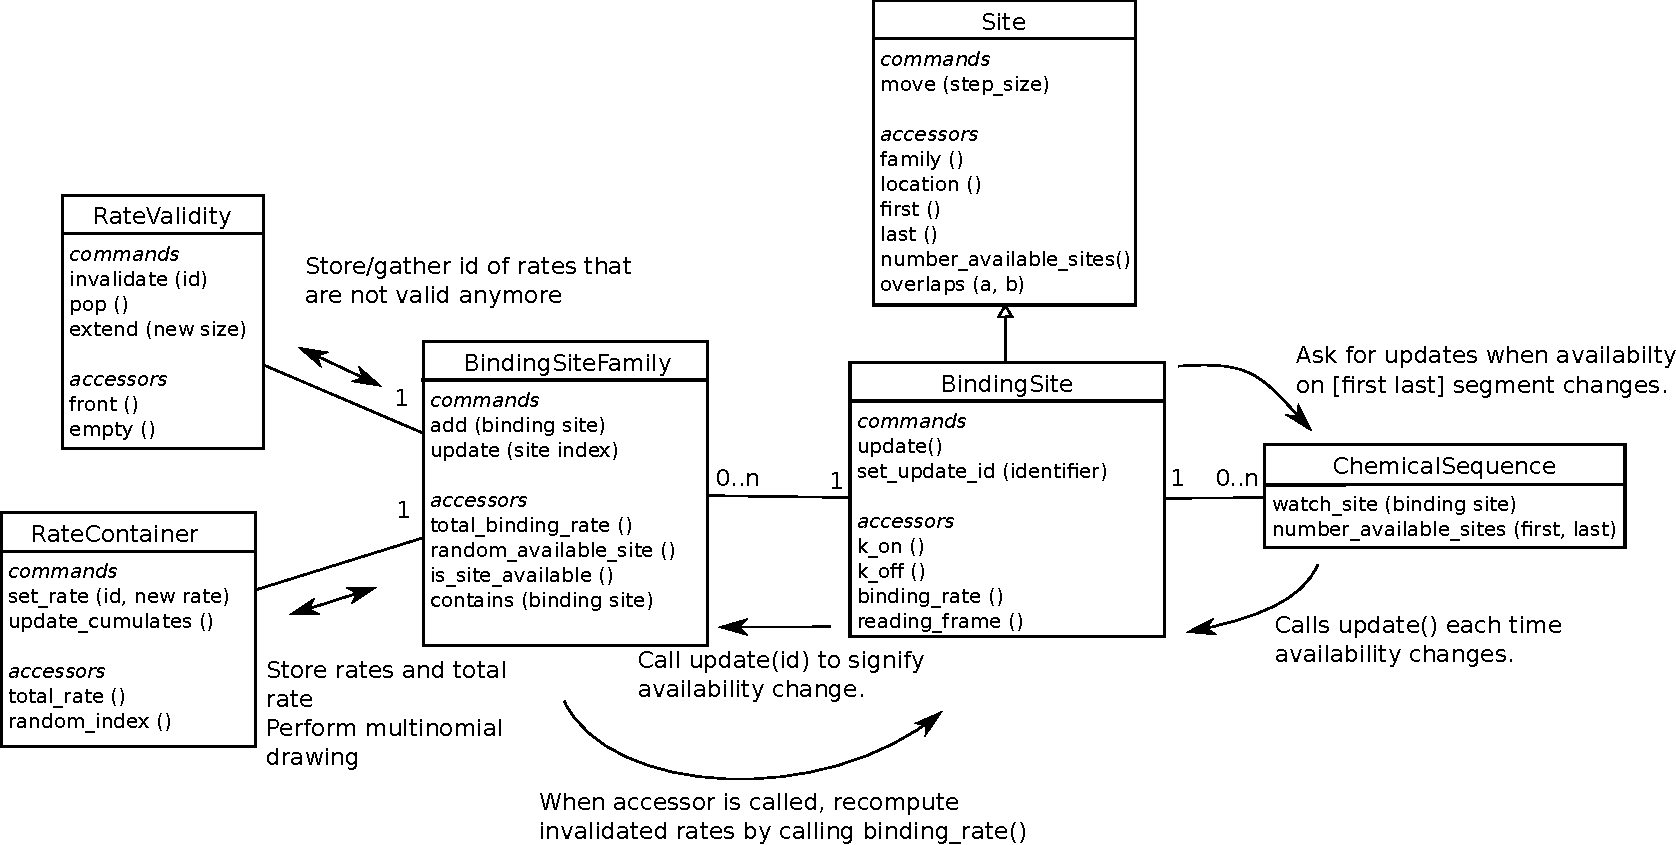
\includegraphics[width=\linewidth]{bindingsitefamily}
  \caption{Schematical view of the Observer pattern used to keep availability of binding sites up to date for \texttt{SequenceBinding} reactions.}
  \label{fig:det_bsf}
\end{figure}

Every \texttt{BindingSite} is viewed as an \emph{observer} by the \texttt{ChemicalSequence} it belongs to. Every time a change occurs on the site, the \texttt{BindingSite} is notified. The latter binding site notifies its \texttt{BindingSiteFamily} using a specific identifier, letting the family know which binding rate is out of date. This information is stored in a \texttt{RateValidity} class. It is only when it is really needed (\textit{i.e.} when a \texttt{SequenceBinding} wants to access total rate or a random site) that rates are recomputed. This avoids useless computations \textit{e.g.} in the case of a translocation, where a bound unit is first unbound from its \texttt{ChemicalSequence} then rebound. If the bound unit does not move away from the site, two updates will be sent, but the rate will only be recomputed once at the end.
